% --
% theory

\section{Theory}\label{sec:nn_theory}
\thesisStateNotReady
The theory provided in this section, merely focuses on the used neural network architectures and some basic theory elements in neural networks.
The most basic element in neural networks is described here as node, an abstract element, usually illustrated as circle, that defines input and output connections from and to other nodes within the network.
The edges of the connections from and to a node represent multiplications with scalar values, denoted as weight.
Each node usually incorporates an additive term, denoted as bias term.
All weights and bias terms are forming the parameters of a network and can be trained through back-propagation.
The output of a node is a scalar computed from all inputs and mapped with a non-linear function denoted as activation function.
A neural network can consist of thousand of nodes in each possible constellation of connections.
In this thesis, the focus is only on single directional connections (no bidirectional connections).
The structure of a neural network is defined by its layers, where a layer is a set of nodes with specific connection properties, that receive inputs from the previous layer and output connections to the next layer.
For example, a neural network consists of one convolutional layer followed by three fully connected layers.
The last layer of a neural network usually represents the class labels of a classification tasks.
A loss function computes the difference between the predicted and the actual class label during training and is essential for the backpropagation algorithm, that updates each parameter in the network through the gradients of the obtained error.


% --
% activation functions

\subsection{Activation Functions}\label{sec:nn_theory_acti}
Activation functions for neural networks of a node in a current layer are non-linear functions that usually maps the sum of the weighted inputs from nodes in a previous layer to a single output value $z$ as following:
\begin{equation}\label{eq:nn_theory_acti}
  z = h(w^T \, x)
\end{equation}
where $h$ is the activation function, $w \in \R^n$ is an weight vector and $x \in \R^n$ an input vector for one specific node.
The output of each node in a current layer is further connected to other nodes in the next layer and builds up the neural network.
The constraint of an activation function is, that an easy computable derivative of this function exist, in order to backpropagate gradients.

The most famous activation function nowadays is the RELU function:
\begin{equation}\label{eq:nn_theory_relu}
  z = \max{(0, a)}
\end{equation}
with $a \in \R$ as input to the activation function.
The big advantage is that this function and its subgradients are very easy and fast to compute.
The two other activation functions that are used in wavenets are the sigmoid function:
\begin{equation}\label{eq:nn_theory_sigmoid}
  z = \frac{1}{1 + \exp{-x}}
\end{equation}
and the tanh functions:
\begin{equation}\label{eq:nn_theory_tanh}
  z = \frac{\exp{x} - \exp{-x}}{\exp{x} + \exp{-x}}
\end{equation}


% --
% fully connected

\subsection{Fully Connected Layer}
A fully connected (FC) layer is one of the simplest and most commonly used layer types in neural network architectures.
Each node from the previous layer is forwardly connected to all nodes in the current FC layer and each node in the current FC layer is connected to all nodes in the next layer.
Further every connection has one trainable weight and every node has a bias term.
A simple FC layer is illustrated in \rfig{nn_theory_fc} with 3 nodes.
% fc
\begin{figure}[!ht]
  \centering
    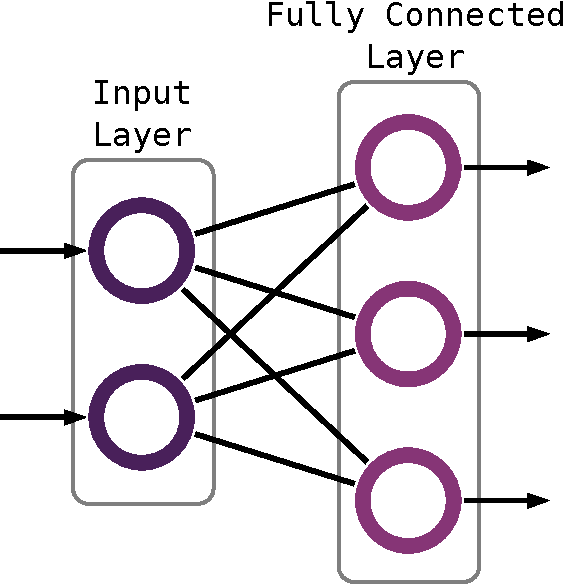
\includegraphics[width=0.30\textwidth]{./4_nn/figs/nn_theory_fc.eps}
  \caption{Basic fully connected layer with 3 nodes, receiving connections from 2 input nodes and outputing connections to 2 output nodes.}
  \label{fig:nn_theory_fc}
\end{figure}
\FloatBarrier
\noindent
Mathematically one node $i$ performs following calculation:
\begin{equation}
  z = h(w^T \, x + b_i)
\end{equation}
with the same notations as described in \req{nn_theory_acti} and an additional bias term $b_i \in \R$.
For all nodes in a layer this equation of a single node can be summarized to a weight matrix $W \in \R^{m \times n}$ with $m$ as total amount of nodes in that layer, so that an FC layer can be written as:
\begin{equation}
  \hat{z} = h(W \, x + b)
\end{equation}
where $b \in \R^m$ are the bias terms of all nodes and $\hat{z} \in \R^m$ the outputs of each nodes in that layer.
With the matrix representation it is easy to obtain the amounts of operations needed for a FC layer.
The amount of parameters are clearly $m \cdot n$ for $W$ and $m$ for $b$ so in total $m \cdot n + m$ parameters.
The amount of operations are the matrix vector multiplication with approximated amounts of multiplication and additions plus the bias terms.
With the activation function disregarded, the amount of calculations are closely:
\begin{equation} 
  \mathcal{T}(W \, x + b) = 2 (m \cdot n) + m
\end{equation}
which would give for example with $n = 128$ and $m = 64$ roughly $\mathcal{T}(W \, x + b) = \SI{16.4}{\kilo\ops}$.


% --
% cnn

\subsection{Convolutional Layers}\label{sec:nn_theory_cnn}
Convolutional layers are the fundamental building block of every Covolutional Neural Networks (CNN), as already discussed in \rsec{prev_nn_cnn}.
Convolutional filters are applied on small areas of the input data, so that spatial information can be retrieved.
Those convolutional filters are also called kernels, denoted as $k$ and illustrated in case of images as rectangles in 2D space with kernel width $d_{k_w}$ and height $d_{k_h}$.
The kernel is shifted over its input map in each dimensional axis with an operation called \emph{stride}, denoted as $s$, and produce an output map through the convolution operation, mathematically denoted with a star $*$.
The output length $d_{o_z}$ of an image in dimension $z$ convoluted from an input length $d_{x_z}$ with a kernel $k$ striding along axis $i$ with $s_z$ and kernel size for that axis $d_{k_z}$ can be computed as following:
\begin{equation}\label{eq:nn_theory_cnn_}
  d_{o_z} = \floor*{\frac{d_{x_z} + p_z - d_{k_z}}{s_z} + 1}
\end{equation}
where $p_z$ is an additional \emph{padding} term in dimension $z$, for instance zero-padding adds zeros on both sides of the selected axis.
For example if a $16 \times 16$ image is convoluted by a $5 \times 5$ kernel with stride $1$ in each direction and no padding is done, the output image is a $12 \times 12$ image.
The padding operation has usually the purpose to keep the same output and input dimension.
This is for instance necessary in residual neural networks, where the input to a residual block with several convolutional layers is bypassed and added to the output of this block again.
Being able to compute the addition operation from input and output of the residual block, their dimensions must coincide.
However in most convolutional network applications without residual blocks, it is preferred not to pad the image, so that dimensions are reduced hence parameters and multiplications saved.
Further some types of sub-sampling layers exist, such as a Max-Pooling layer, especially designed to reduce the dimensions of the output image and save computations.

A convolutional layer is defined by the amount of input and output channels (feature maps), the kernel size, the stride of the kernel and some other specialties like dilation.
However it is not immediately clear from those parameter, how many convolutional filters are applied and how the output feature maps are calculated exactly.
The amount of convolutional filters $k$ is in most practical examples always:
\begin{equation}\label{eq:nn_theory_n_filters}
  \#k = i \cdot j
\end{equation}
where $i$ and $j$ is the amount of input and output channels respectively.
Each kernel produces an output map, but the idea is to constraint the number of output maps $\#k$ to the defined output channels $j$.
This is usually done by summing up all output maps of input channels $i$ for one output channel $j$:
\begin{equation}
  o_j = \sum_{i} k_{i, j} * x_i
\end{equation}
where $o_j$ is the j-th feature map, $k_{i, j}$ the kernel of $i$ and $j$ and $x_i$ the i-th input channel.
A graphical example of this procedure is shown in \rfig{nn_theory_cnn_basics}.
% cnn basics
\begin{figure}[!ht]
  \centering
    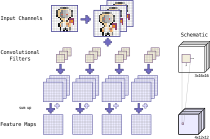
\includegraphics[width=0.6\textwidth]{./4_nn/figs/nn_theory_cnn_basics.eps}
  \caption{Basic CNN layer with a $16 \times 16$ input image, decomposed in 3 channels (CYM) and 4 output feature maps. Kernel size is $5 \times 5$ and the stride is $1$.}
  \label{fig:nn_theory_cnn_basics}
\end{figure}
\FloatBarrier
\noindent

The amount of parameters are all weights in the convolutional filters (kernels) and their bias terms, however the bias terms for each filter can be ignored, in this thesis no bias terms were used for the convolutional layers.
Therefore the amount of parameters are $\#k \cdot d_{k_w} \cdot d_{k_h}$ for a two dimensional convolutional layer, which makes $3 \cdot 4 \cdot 5 \cdot 5 = 300$ parameters for the example in \rfig{nn_theory_cnn_basics}.
The amount of operations are therefore each convolution operation for each filter and the summation to $j$ output channels.
One convolution with a single two dimensional kernel $k$ and one input channel $x$ has an approximate number of multiplication and addition operations:
\begin{equation}
  \mathcal{T}(k * x) = 2(d_{k_w} \cdot d_{k_h}) (d_{o_w} \cdot d_{o_h})
\end{equation}
and for all feature maps and the summation of them to the output channels:
\begin{equation}
  \mathcal{T}(o) = \#k \cdot \mathcal{T}(k * x) + \#k \cdot (d_{o_w} \cdot d_{o_h})
\end{equation}
For the previous example this would give $\mathcal{T}(k * x) = 2 (12 \cdot 12) (5 \cdot 5) = \SI{7.2}{\kilo\ops}$ and $\mathcal{T}(o) = 12 \cdot \SI{7.2}{\kilo\ops} + 12 \cdot (12 \cdot 12) = \SI{88.1}{\kilo\ops}$.




% --
% loss functions

\subsection{Loss Functions and Softmax}
Loss functions also known as cost functions are used to determine the difference between the predicted labels $\hat{y}$ compared to the actual or ground truth labels $y$.
The predicted labels are usually presented by the output nodes in the last layer of a neural network.
Therefore $\hat{y} = [\hat{y_1}, \, \hat{y_2}, \dots, \hat{y_c}]^T$ has the dimension of the number of labels or classes $c$.
Often it is preferred that $\hat{y} \in R^c$ provides a probability distribution such that:
\begin{equation}
  \sum_{i=0}^c \hat{y}_i = 1
\end{equation}
which can be achieved with the softmax function:
\begin{equation}\label{eq:nn_theory_softmax}
  \hat{y}_i = \frac{\exp{x_i}}{\sum_{j=0}^{c}\exp{x_j}}
\end{equation}
where $c$ is the amount of nodes in this layer, if it is the last layer as usual for the softmax, $c$ is the amount of classes and $\hat{y}_i$ the probability value of the corresponding class $i$.

There are already plenty of different loss functions available for training neural networks, however in this thesis only one kind of it is used for all neural network architecture, the cross-entropy loss or for two classes the binary cross-entropy loss function.
Without going too much into the detail of this loss function, it is described in the same way as in the \texttt{pytorch} framework \cite{Pytorch}.
The binary cross entropy is implemented as:
\begin{equation}
  l_i(x_i, y_i) = y_i \cdot \log x_i + (1 - y_i) \cdot \log (1 - x_i)
\end{equation}
where $n$ is the sample index of the training pair $(x_i, y_i)$, with $x_i$ as feature input and $y_i$ as corresponding label.
During the training procedure a whole batch of sample size $N$ is sent through the network for classification.
The loss function should provide only a single value, therefore all $l_i$ with $i = 0, \dots, N$ must be concatenated.
This can simply be done for instance with the calculation of the mean of all $l_i$.


% --
% dropout

\subsection{Dropout}
Dropout \cite{Hinton2012} is a method to improve generalization and training of neural networks.
The idea is to set the output of randomly selected nodes within a layer for one training step to zero, so that only the other nodes are updated.
This can be done by multiplying all outputs of a current layer with a vector containing a specified number of zeros and ones places at random positions within the vector.
The amount of zeros compared to ones can be sampled from a Bernoulli distribution set by a probability value, for instance $p=0.2$ means that there are 20\% zeros and 80\% ones randomly placed within the vector.


% --
% training

\subsection{Training of a Neural Network}
The training of a neural network is usually done by updating each parameter of the model with back-propagated gradients from the loss obtained at the output nodes.
The loss is calculated by a specific loss function comparing the predicted labels to the targets of the actual training samples.
To update the parameters of the network, an update rule, such as Stochastic Gradient Descend (SGD) or Adam \cite{Kingma2015} is applied.
Note that a single update step is usually not performed on the whole dataset, unless it is a very small dataset. 
In the normal case the update is performed for each small chunk of the dataset called \emph{batch}.
During one training iteration, denoted as \emph{epoch}, each example in the dataset is processed a single time, then the next epochs starts.
Note that the training of neural networks may take over thousands of epochs until a convergence is reached.
The general training techniques for neural networks and further details are not described here, because of many existing books and papers \cite{LeCun2006}, \cite{Goodfellow2016}, \cite{DeepLearning} that are already presenting this topic very well. 
Further it does not add any value to this thesis as the algorithms are well examined and run in the background of all neural network frameworks.
The interesting elements are therefore only the neural network architecture design, the training parameters and the used loss functions.
